\documentclass[11pt,letterpaper]{article}
%% This is roots-vig.Rnw
%\VignetteIndexEntry{Examples of 1D rootfinding in R}
\usepackage[american]{babel}
\usepackage[utf8]{inputenc}
\newcommand{\R}{{\sf R\ }}
\newcommand{\Splus}{{\sf S-PLUS}}
\newcommand{\fixme}[1]{\textbf{FIXME: #1}}
%\newcommand{\fixme}[1]{}
\newcommand{\code}[1]{{\tt #1}}
\providecommand{\pkg}[1]{{\fontseries{b}\selectfont #1}}
\let\proglang=\textsf
\usepackage{url}
%%\usepackage{natbib}
\usepackage{listings}
\usepackage{verbatim}
\usepackage{Sweave}

\usepackage{graphicx} %If you want to include postscript graphics
\bibliographystyle{amsplain}

\begin{document}
\Sconcordance{concordance:roots-vig.tex:roots-vig.Rnw:%
1 92 1 1 2 1 0 1 7 6 0 2 1 5 0 2 1 19 0 5 1 6 0 1 2 3 1 1 2 1 0 2 1 19 %
0 4 1 6 0 1 2 2 1 1 2 1 0 2 1 19 0 4 1 6 0 1 2 2 1 1 2 1 0 2 1 19 0 4 1 %
6 0 1 2 28 1 1 2 1 0 2 1 19 0 4 1 5 0 1 2 5 0 2 1 19 0 2 1 6 0 1 2 16 1 %
1 2 1 0 1 3 2 0 2 1 18 0 4 1 5 0 4 1 9 0 1 3 10 1 1 2 1 0 1 3 2 0 2 1 %
18 0 4 1 5 0 4 1 9 0 1 3 12 1 1 2 6 0 1 4 3 0 1 2 5 0 3 1 18 0 1 1 5 0 %
2 1 19 0 1 2 35 1 1 2 6 0 1 4 3 0 8 1 10 0 1 2 21 1 1 2 1 0 1 9 8 0 2 1 %
5 0 1 1 5 0 3 1 5 0 1 1 5 0 2 1 19 0 1 2 11 1 1 2 1 0 1 3 2 0 2 1 5 0 1 %
1 5 0 3 1 5 0 1 1 5 0 2 1 9 0 1 1 5 0 4 1 5 0 2 1 19 0 1 2 46 1 1 19 18 %
0 1 3 2 0 1 9 37 0 1 2 17 1 1 2 6 0 10 1 5 0 1 2 6 0 3 1 27 0 2 1 5 0 1 %
2 8 0 1 2 132 1}


\title{Roots of Functions of One Variable in \R}
\author{John C. Nash\\ Telfer School of Management\\ University of Ottawa\\Ottawa, Canada}
\date{October 2011}
\maketitle

\section*{Abstract}


This vignette is intended to show how problems that devolve into finding the root(s) of a function
of one variable may arise and how \R  may solve them. We will mention polynomial root-finding, but 
generally regard this (and eigenvalues of matrices) to be somewhat different problems from those that
will be the focus here. 

We also wish to point out the limitations of computational technology for root-finding. Treating
root-finders as black boxes is, in the author's view, dangerous in that it risks many possibilities for poor approximations to the answers we desire, or even drastically wrong answers. Largely this is because users may make assumptions about the problem and/or the software that are not justified.  Indeed, in this vignette we mostly seek only real-valued solutions to equations. 

Finally we want to show that the built-in tool for one-dimensional root-finding in \R  (\texttt{uniroot}), while a very good choice, is still based on several design considerations that may not be a good fit to particular user problems.

\section{Equations in one variable}

There are many mathematical problems stated as equations. If we have one equation and only one variable in the equation is "unknown", that is, not yet determined, then we should be able to solve the equation. In order to do this, we shall specify that the unknown variable is $x$ and rewrite the equation as

$f(x) = 0$

Of course, there may be more than one value of $x$ that causes $f(x)$ to be zero. This multiplicity of solutions is one of the principal difficulties for rootfinding software. 
Roots might also have complex values, and it is quite reasonable that users (and software) may consider that only real roots are admissible and wanted. 


\section{Some examples}


In this section, we look at some examples which illustrate some particular issues that are 
relevant to rootfinding software and its usage.

\subsection{An extra foot}

This is a problem from \cite{acton70} .


\begin{quote}
SPMA terrorists find a 1 mile section of welded rail that is pinned at each end. In one of the two rails (Stephenson gauge), they weld an extra foot of rail. If that rail bows away from its partner in a regular circular arc, how far apart are the rails at the widest point?
\end{quote}

The problem can be drawn as follows:

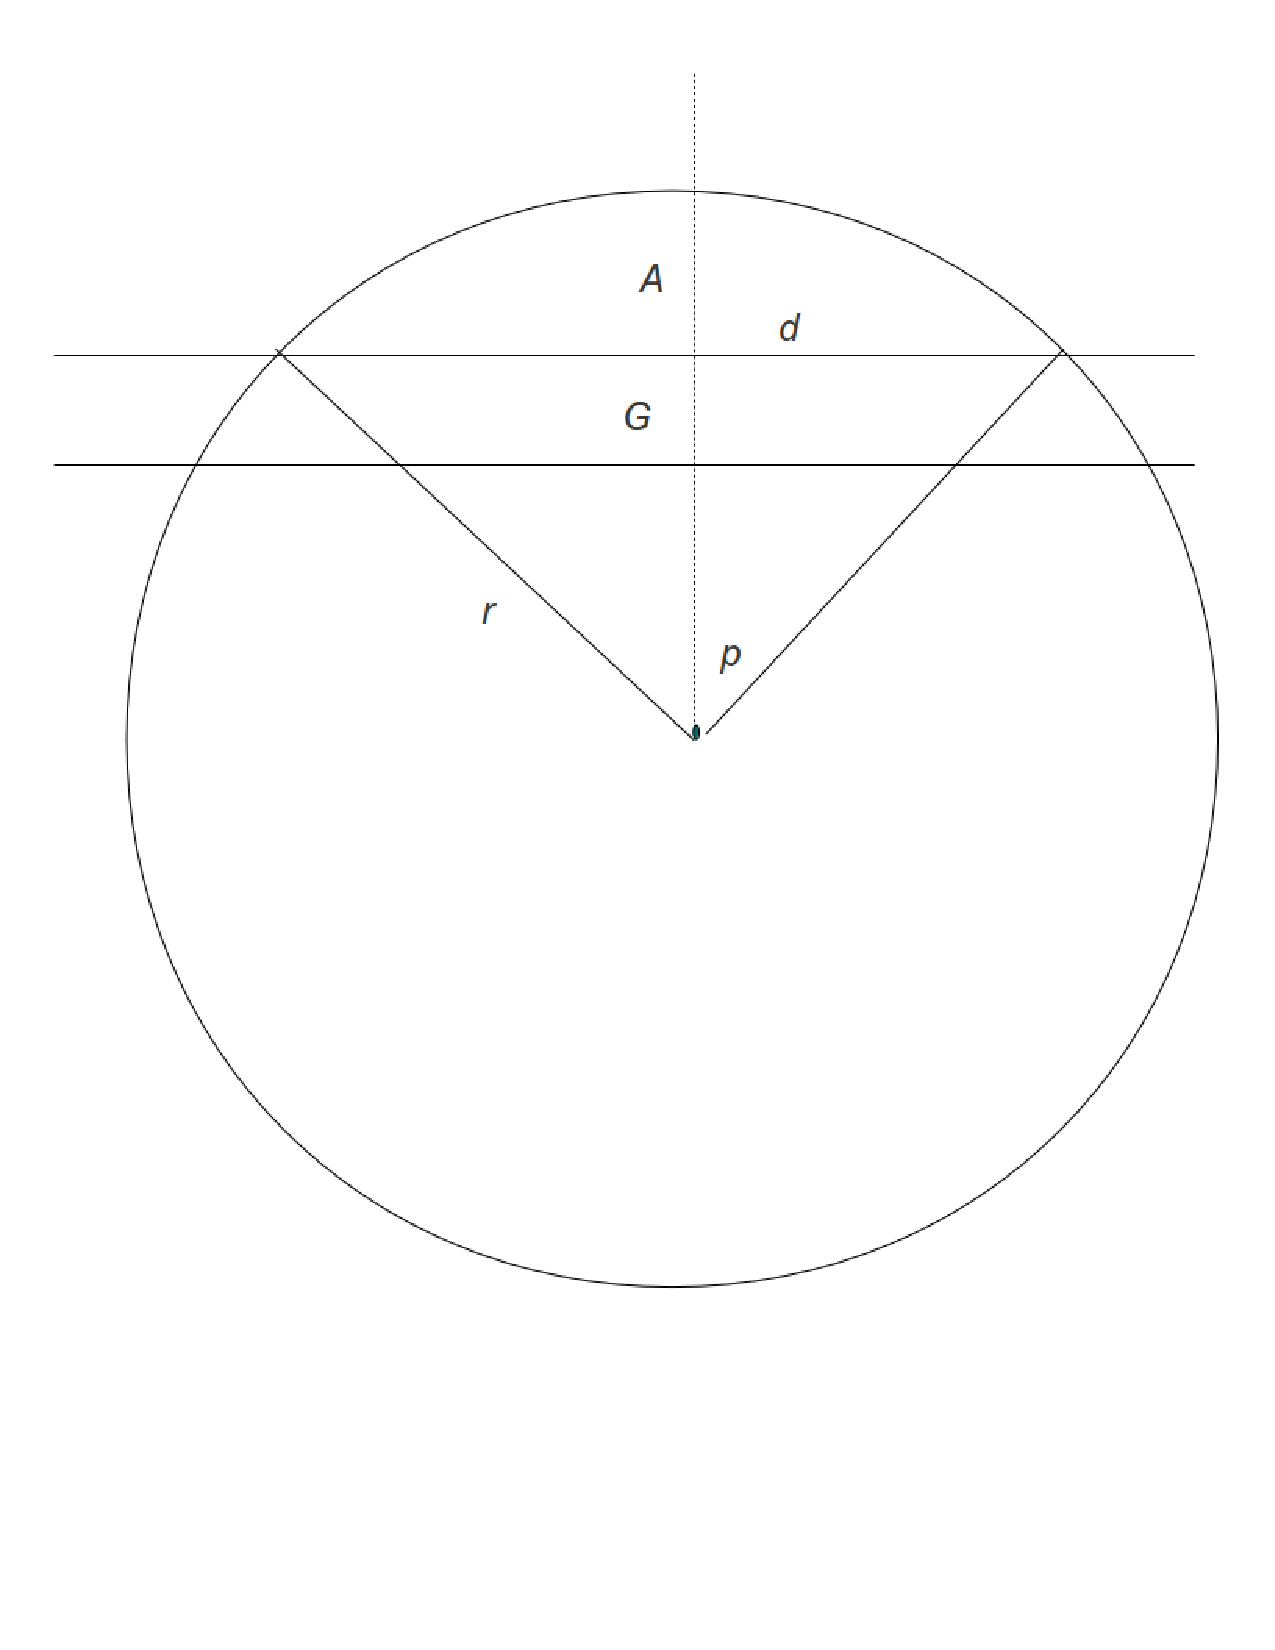
\includegraphics[height=3.5in, width=3in]{onefoot.pdf} 

Our goal is to compute $A+G$. If we presume Standard (Stephenson) gauge, then $G$ = 4 feet 8.5 inches. (Acton has given us Imperial measurements to complicate the task). Thus $G$ = 4 + 17/24 feet. The distance $d$ is 0.5 * 5280 = 2640 feet, and the arc above it is 0.5 * 5281 = 2640.5 feet. If the angle $p$ is in radians, we then get the two equations for the radius $r$ of the circular arc and the angle $p$

$ r * p = 2640.5 $  

and

$ r * sin(p) = 2640 $

There we are: 2 equations in 2 unknowns. "Piece of cake" comes to mind. Hold on! These are not so easy to solve.

First, we could solve them both at once by defining a sum of squares function of the residuals

\indent
$ e1 = r * p - 2640.5 $\\
\indent
$ e2 = r * sin(p) - 2640 $

\noindent
as  $ sumsq(r, p) = e1^2 + e2^2 $

\R  provides a reasonable way to do this with the optim() function and its Nelder-Mead default method. We simply need some sort of starting values and our $sumsq()$ function. As a start, let us assume that the radius $r$ will be at least a few miles. Try 20000 feet. And the angle p should be at least some fraction of a radian, so let us try 0.5. (These are quite poor estimates; we can do much better just using Pythagorus' theorem.)

\begin{Schunk}
\begin{Sinput}
> rm(list=ls())
> railss<-function(xx){ # SPMA rail problem to provide sumsquares of residuals
+     r<-xx[1]
+     p<-xx[2] # get the two parameters
+     e1<-r*sin(p)-2640
+     e2<-r*p-2640.5
+     ss<-e1*e1+e2*e2
+ }
> x<-c(10000, 0.5) # start
> cat("Function at start = ",railss(x),"\n")
\end{Sinput}
\begin{Soutput}
Function at start =  10208057 
\end{Soutput}
\begin{Sinput}
> ans<-optim(x, railss)
> print(ans)
\end{Sinput}
\begin{Soutput}
$par
[1] 1.290627e+04 2.051969e-01

$value
[1] 165.6857

$counts
function gradient 
     207       NA 

$convergence
[1] 0

$message
NULL
\end{Soutput}
\begin{Sinput}
> rr<-ans$par[1]
> pp<-ans$par[2]
> GG<-4 + 8.5/12
> AA<-  rr*(1-cos(pp)) 
> cat("rail distance = ",AA," + G =",AA+GG,"\n")
\end{Sinput}
\begin{Soutput}
rail distance =  270.7622  + G = 275.4706 
\end{Soutput}
\end{Schunk}

This "answer" is not, however, very good. Note that the value of the function at the finish -- a sum of squares that should be zero -- is 165. This is a result of a very large initial function, of the order of 1E+7, which scales the convergence tolerances. However, we can restart from the finish point of the "first try". 


\begin{Schunk}
\begin{Sinput}
> xx<-ans$par # new start
> ans2<-optim(xx, railss)
> print(ans2)
\end{Sinput}
\begin{Soutput}
$par
[1] 2.398158e+04 1.101986e-01

$value
[1] 11.80843

$counts
function gradient 
     501       NA 

$convergence
[1] 1

$message
NULL
\end{Soutput}
\begin{Sinput}
> rr<-ans2$par[1]
> pp<-ans2$par[2]
> AA<-rr*(1-cos(pp)) 
> cat("rail distance = ",AA," + G =",AA+GG,"\n")
\end{Sinput}
\begin{Soutput}
rail distance =  145.4657  + G = 150.1741 
\end{Soutput}
\end{Schunk}

This time we have exceeded the function evaluation limit of 500. We can fix this easily if we don't mind making our computer work a bit. 

\begin{Schunk}
\begin{Sinput}
> xx<-ans$par # new start
> ans2<-optim(xx, railss, control=list(maxit=20000))
> print(ans2)
\end{Sinput}
\begin{Soutput}
$par
[1] 4.936003e+04 5.350205e-02

$value
[1] 0.2891659

$counts
function gradient 
    1837       NA 

$convergence
[1] 0

$message
NULL
\end{Soutput}
\begin{Sinput}
> rr<-ans2$par[1]
> pp<-ans2$par[2]
> AA<-rr*(1-cos(pp)) 
> cat("rail distance = ",AA," + G =",AA+GG,"\n")
\end{Sinput}
\begin{Soutput}
rail distance =  70.62894  + G = 75.33727 
\end{Soutput}
\end{Schunk}

Better, but the sum of squares is still not zero. We could try a different optimizer.

\begin{Schunk}
\begin{Sinput}
> xx<-ans$par # new start
> ans3<-optim(xx, railss, method='BFGS', control=list(maxit=20000))
> print(ans3)
\end{Sinput}
\begin{Soutput}
$par
[1] 1.835054e+04 1.441258e-01

$value
[1] 37.38682

$counts
function gradient 
   72002    20000 

$convergence
[1] 1

$message
NULL
\end{Soutput}
\begin{Sinput}
> rr<-ans3$par[1]
> pp<-ans3$par[2]
> AA<-rr*(1-cos(pp)) 
> cat("rail distance = ",AA," + G =",AA+GG,"\n")
\end{Sinput}
\begin{Soutput}
rail distance =  190.2613  + G = 194.9697 
\end{Soutput}
\end{Schunk}

None of these answers are very good. Indeed, let us abandon for the moment the "circular
arc" and simply use a triangular approximation as in the figure below. 


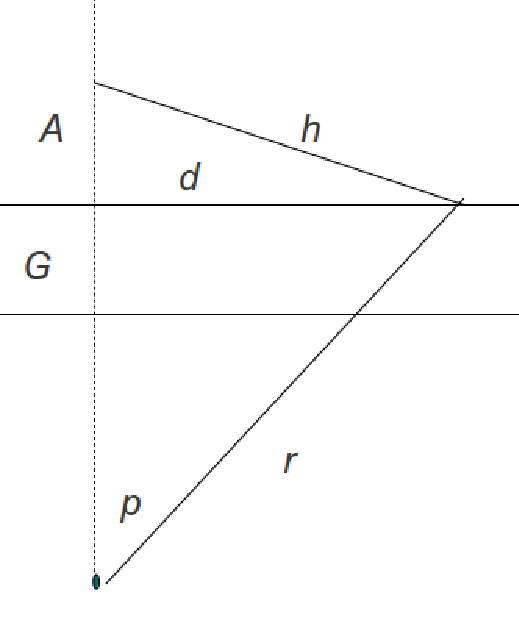
\includegraphics[height=3in, width=2.6in]{onefootb.pdf}

Then the Pythagorean rule gives us 

$ A = sqrt(2640.5^2 - 2640^2) $

or approximately 51.38 feet. 

Using Pythagorus again, we find

$  (r-A)^2 + 2640^2 = r^2 $

or

$ 2*r*A = 2640^2  + A^2 $

giving, $r$ approximately 67845.3 feet. In turn, this gives $p$ as

$  p = 2640.5/r $  

or 0.03892 radians, about 2.23 degrees.

Starting our optimization from $r$ = 70000 and $p$ = .04 gives.

\begin{Schunk}
\begin{Sinput}
> xy<-c(70000, .04) # new start
> ans4<-optim(xy, railss, control=list(maxit=20000))
> print(ans4)
\end{Sinput}
\begin{Soutput}
$par
[1] 7.268903e+04 3.632673e-02

$value
[1] 0.003682029

$counts
function gradient 
      85       NA 

$convergence
[1] 0

$message
NULL
\end{Soutput}
\begin{Sinput}
> rr<-ans4$par[1]
> pp<-ans4$par[2]
> AA<-rr*(1-cos(pp)) 
> cat("rail distance = ",AA," + G =",AA+GG,"\n")
\end{Sinput}
\begin{Soutput}
rail distance =  47.95609  + G = 52.66442 
\end{Soutput}
\begin{Sinput}
> cat("\n Try from last solution")
\end{Sinput}
\begin{Soutput}
 Try from last solution
\end{Soutput}
\begin{Sinput}
> ans5<-optim(c(rr, pp), railss, control=list(maxit=20000))
> print(ans5)
\end{Sinput}
\begin{Soutput}
$par
[1] 7.833505e+04 3.370777e-02

$value
[1] 1.796436e-13

$counts
function gradient 
    1127       NA 

$convergence
[1] 0

$message
NULL
\end{Soutput}
\begin{Sinput}
> AA<-rr*(1-cos(pp)) 
> cat("rail distance = ",AA," + G =",AA+GG,"\n")
\end{Sinput}
\begin{Soutput}
rail distance =  47.95609  + G = 52.66442 
\end{Soutput}
\end{Schunk}

The last answer is actually quite good. And we \textbf{know} that it is a good
answer because the sum of squares is very small. This is the \textbf{value} element
of the optimization answer.

Our second solution is to substitute $ r = 2640.5/p $ from the first of our equations
into the second, giving

$ 2640.5 * sin(p)/p - 2640 = g(p) = 0 $

We seek roots of $g(p)$, and \R   offers us \texttt{uniroot()}, which requires us to 
provide an interval estimate for the location of a root. Moreover, g(p) should have 
opposite signs at each end of the interval. Let us choose $p$ in [0.01, 0.1]. That 
this is a good choice is shown by the graph of the function.

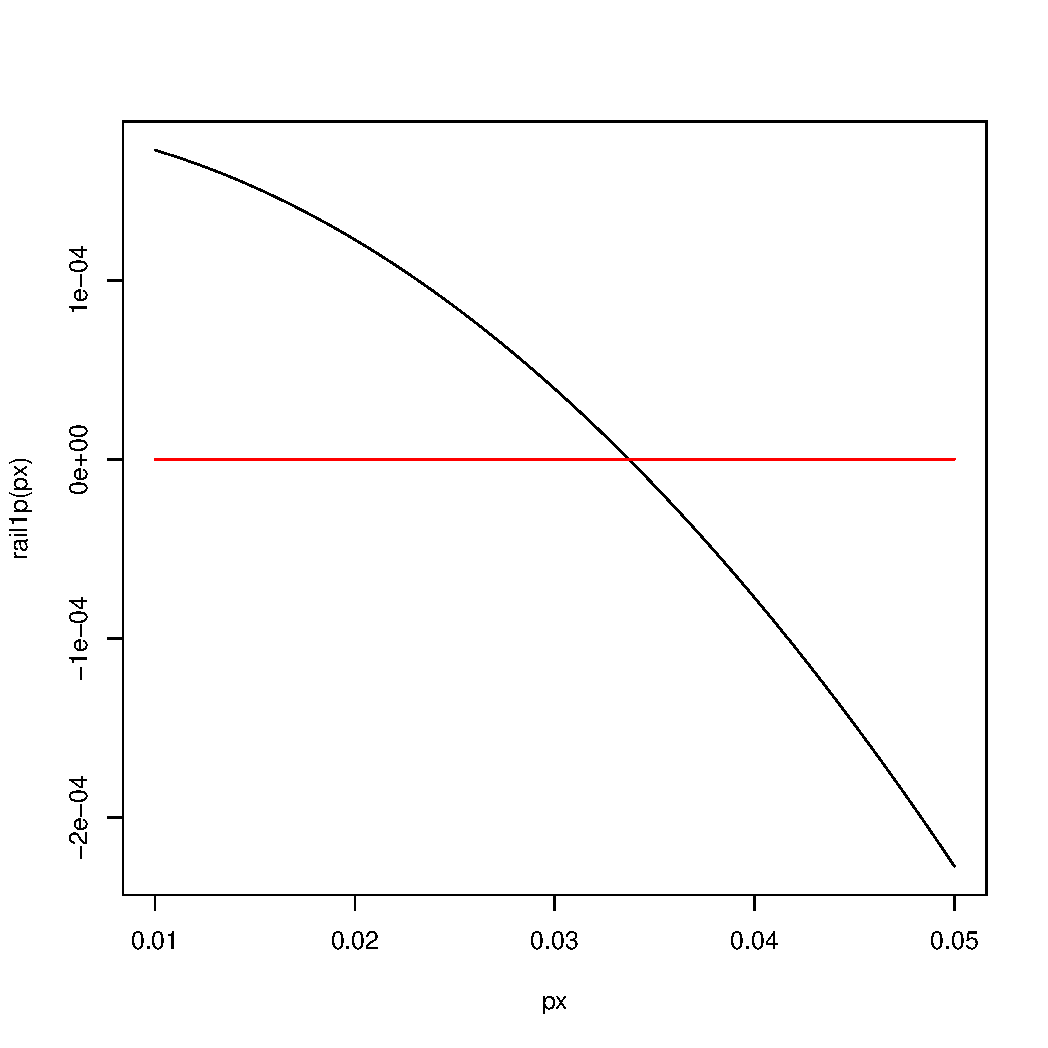
\includegraphics[height=3in]{rail1p.pdf}

\begin{Schunk}
\begin{Sinput}
> tint<-c(0.01, 0.1) # interval for root
> g<-function(p) {
+  fun<-2640.5 * sin(p)/p - 2640
+ }
> tryp<- uniroot(g, tint)
> print(tryp)
\end{Sinput}
\begin{Soutput}
$root
[1] 0.0337213

$f.root
[1] -0.0004018539

$iter
[1] 7

$init.it
[1] NA

$estim.prec
[1] 6.103516e-05
\end{Soutput}
\begin{Sinput}
> pp<-tryp$root
> rr <- 2640.5/pp
> AA<-rr*(1-cos(pp)) 
> cat("rail distance = ",AA," + G =",AA+GG,"\n")
\end{Sinput}
\begin{Soutput}
rail distance =  44.51633  + G = 49.22466 
\end{Soutput}
\begin{Sinput}
> e1<-rr*sin(pp)-2640
> e2<-rr*pp-2640.5
> ss<-e1*e1+e2*e2
> cat("ss loss function = ", ss, "\n")
\end{Sinput}
\begin{Soutput}
ss loss function =  1.614865e-07 
\end{Soutput}
\begin{Sinput}
> 
\end{Sinput}
\end{Schunk}

This is "not too bad". 

Our third approach solves using $r$, that is, 

$ r * sin(2640.5/r) - 2640 = f(r) = 0 $

We choose a fairly wide interval in which to search for a root.

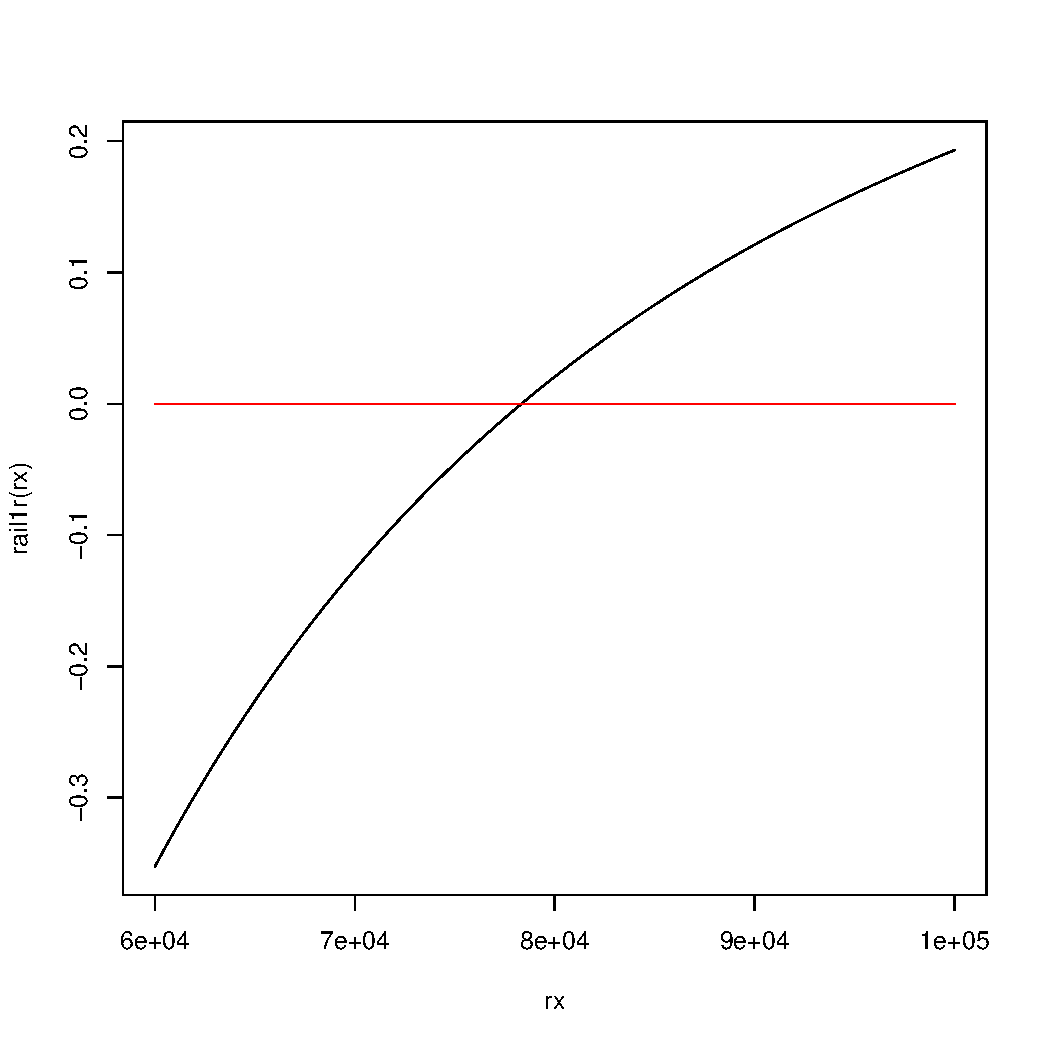
\includegraphics[height=3in]{rail1r.pdf}

\begin{Schunk}
\begin{Sinput}
> tinr<-c(50000, 90000) # interval for root
> f<-function(r) {
+  fun<-r * sin(2640.5/r) - 2640
+ }
> tryr<- uniroot(f, tinr)
> print(tryr)
\end{Sinput}
\begin{Soutput}
$root
[1] 78335.08

$f.root
[1] 0

$iter
[1] 7

$init.it
[1] NA

$estim.prec
[1] 33.47549
\end{Soutput}
\begin{Sinput}
> rr<-tryr$root
> pp <- 2640.5/rr
> AA<-rr*(1-cos(pp)) 
> cat("rail distance = ",AA," + G =",AA+GG,"\n")
\end{Sinput}
\begin{Soutput}
rail distance =  44.49846  + G = 49.20679 
\end{Soutput}
\begin{Sinput}
> e1<-rr*sin(pp)-2640
> e2<-rr*pp-2640.5
> ss<-e1*e1+e2*e2
> cat("ss loss function = ", ss, "\n")
\end{Sinput}
\begin{Soutput}
ss loss function =  0 
\end{Soutput}
\begin{Sinput}
> 
\end{Sinput}
\end{Schunk}

We are not going to get a better sum of squares than 0.

\subsection{Not there!}

An issue to which we will return later concerns the possibility that we have
a function $f(x)$ that becomes singular at some point $x$. A nice example is
the tangent of an angle. For convenience, let us measure the angle in degrees,
so for  \R  we modify the internal function so the argument is appropriately
scaled by $180/pi$ (see the code chunk). Now if we consider this function from
80 to 100 degrees, we get a curve approaching +Infinity from below and -Infinity
from above (i.e., larger angles). There is no root at 90 degrees. However, ...

\begin{Schunk}
\begin{Sinput}
> cat("Tangent function false root\n")
\end{Sinput}
\begin{Soutput}
Tangent function false root
\end{Soutput}
\begin{Sinput}
> mytan<-function(xdeg){ # tangent in degrees
+     xrad<-xdeg*pi/180.0 # conversion to radians
+     tt<-tan(xrad)
+ }
> cat("find root between 80 and 100 degrees\n")
\end{Sinput}
\begin{Soutput}
find root between 80 and 100 degrees
\end{Soutput}
\begin{Sinput}
> tint<-c(80,100)
> rtan1<-uniroot(mytan, tint)
> print(rtan1)
\end{Sinput}
\begin{Soutput}
$root
[1] 90.00008

$f.root
[1] -750991.8

$iter
[1] 19

$init.it
[1] NA

$estim.prec
[1] 7.629348e-05
\end{Soutput}
\begin{Sinput}
> cat("\n\nTighten the tolerance\n")
\end{Sinput}
\begin{Soutput}
Tighten the tolerance
\end{Soutput}
\begin{Sinput}
> rtan2<-uniroot(mytan, tint, tol=.Machine$double.eps)
> print(rtan2)
\end{Sinput}
\begin{Soutput}
$root
[1] 90

$f.root
[1] -7.867602e+14

$iter
[1] 49

$init.it
[1] NA

$estim.prec
[1] 7.105427e-14
\end{Soutput}
\end{Schunk}

This is unfortunate. It is a reminder to check our solutions, which in this case
is easily done with a graph. Also we might consider the large size of the function
at the root to be a hint of trouble, but this is not necessarily a conclusive 
indicator. Later we will consider some ways we might make our
rootfinders provide some warnings.


\subsection{A normal concern}

The tangent is an obvious case where the function values are going "away" from 
zero as we approach the root, so we might think that such behaviour could be
used as an indicator of trouble. However, it is possible to have functions that
look somewhat like the tangent but still actually have roots. In fact, we may 
find other difficulties as well. Consider the Gaussian (normal) density function

%% How to improve spacing and font-sizes?
$ f(x) = \frac{1}{sqrt(2 * pi * sigma^2) } exp(-0.5*((x - mu)/sigma)^2) $


This is the usual "bell shaped" curve. It is always positive, so not a function
for which we want to find roots. However, its derivative with respect to x has 
the right properties. This can be found using \R with the \texttt{D()} function. 
The function we want to use is 


$ g(x) = \frac{-1}{sqrt(2 * pi * sigma^2))} *  \frac{(x - mu)}{sigma^2} exp(-(x - mu)^2/(2 * sigma^2)  $


Let us set mu = 4 and draw the function from 0 to 8 for $sigma = 1$ (in red) and $sigma = 0.1$.
To keep the graph viewable, we graph the log of the magnitudes, but keep the sign. As the standard deviation sigma gets smaller, the function gets steeper.

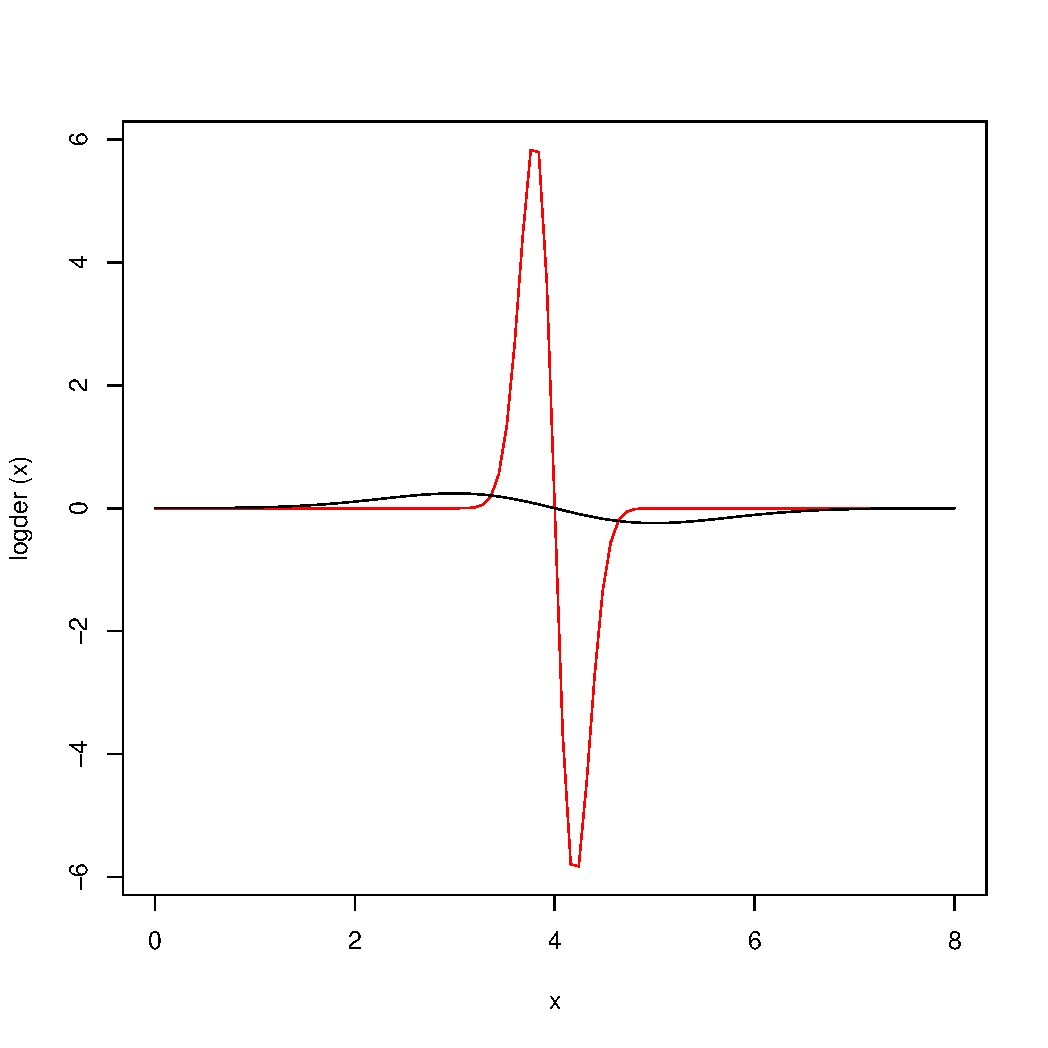
\includegraphics[height=4in, width=5in]{logder.pdf}

Let us use 2 and 6 as the limits of our search interval and find the root for $sigma$ progressively smaller. 

\begin{Schunk}
\begin{Sinput}
> cat("Gaussian derivative\n")
\end{Sinput}
\begin{Soutput}
Gaussian derivative
\end{Soutput}
\begin{Sinput}
> der<-function(x,mu,sigma){
+     dd<-(-1)*(1/sqrt(2 * pi * sigma^2)) * (exp(-(x - mu)^2/(2 * sigma^2)) * 
+     ((x - mu)/(sigma^2)))
+ }
> r1<-uniroot(der, lower=2, upper=6, mu=4, sigma=1)
> r.1<-uniroot(der, lower=2, upper=6, mu=4, sigma=.1)
> r.01<-uniroot(der, lower=2, upper=6, mu=4, sigma=.01)
> r.001<-uniroot(der, lower=2, upper=6, mu=4, sigma=.001)
> sig<-c(1, .1, .01, .001)
> roo<-c(r1$root, r.1$root, r.01$root, r.001$root)
> tabl<-data.frame(sig, roo)
> print(tabl)
\end{Sinput}
\begin{Soutput}
    sig roo
1 1.000   4
2 0.100   4
3 0.010   2
4 0.001   2
\end{Soutput}
\end{Schunk}

What is going on here?! We know the root should be at 4, but in the final two 
cases it is at 2. The reason turns out to be that the function value at $x=2$ is
computationally zero -- a root. The danger is that we just don't recognize that 
this is not the "root" we likely wish to find, for example, if we are using the
derivative as a way to sharpen the finding of a peak on a spectrometer. 

\subsection{Little Polly Nomial}

Polynomial roots are a common problem that should generally be solved by methods
different from those of interest here. We are really only looking at methods to find
a single real root of a real scalar function of one variable. This is easily illustrated
by an example. Suppose we want the roots of the polynomial

$  z(x) = 10 - 3 * x + x^3 $

This has the set of coefficients that we would establish using the \R  code

\texttt{ z <- c(10, -3, 0, 1) }

The package \texttt{polynom} solves this easily using \texttt{polyroot(z)}.

\begin{Schunk}
\begin{Sinput}
> z <- c(10, -3, 0, 1)
> simpol<-function(x){ # calculate polynomial z at x 
+    zz <- c(10, -3, 0, 1)
+    ndeg<-length(zz)-1 # degree of polynomial
+    val<-zz[ndeg+1]
+    for (i in 1:ndeg){
+        val<-val*x+zz[ndeg+1-i]
+    }
+    val
+ }
> tint<-c(-5,5)
> cat("roots of polynomial specified by ")
\end{Sinput}
\begin{Soutput}
roots of polynomial specified by 
\end{Soutput}
\begin{Sinput}
> print(z)
\end{Sinput}
\begin{Soutput}
[1] 10 -3  0  1
\end{Soutput}
\begin{Sinput}
> require(polynom)
> allroots<-polyroot(z)
> print(allroots)
\end{Sinput}
\begin{Soutput}
[1]  1.306444+1.456155i -2.612888+0.000000i  1.306444-1.456155i
\end{Soutput}
\begin{Sinput}
> cat("single root from uniroot on interval ",tint[1],",",tint[2],"\n")
\end{Sinput}
\begin{Soutput}
single root from uniroot on interval  -5 , 5 
\end{Soutput}
\begin{Sinput}
> rt1<-uniroot(simpol, tint)
> print(rt1)
\end{Sinput}
\begin{Soutput}
$root
[1] -2.612888

$f.root
[1] 2.532119e-06

$iter
[1] 9

$init.it
[1] NA

$estim.prec
[1] 6.103516e-05
\end{Soutput}
\end{Schunk}

Here we see that uniroot does a perfectly good job of finding the real root
of this cubic polynomial. It will not, however, solve the simple polynomial

$ y(x) = (x-4)^2 $

because the roots are both at 4 and the function never crosses the $y$ axis. 
\texttt{uniroot} insists on having a starting interval where the function has
opposite sign at the ends of the interval. Uniroot should (and in our example
below does) work when there is a root with odd multiplicity, so that there is
a crossing of the axis.

\begin{Schunk}
\begin{Sinput}
> z <- c(16, -8, 1)
> simpol2<-function(x){ # calculate polynomial z at x 
+    val <- (x-4)^2
+ }
> tint<-c(-5,5)
> cat("roots of polynomial specified by ")
\end{Sinput}
\begin{Soutput}
roots of polynomial specified by 
\end{Soutput}
\begin{Sinput}
> print(z)
\end{Sinput}
\begin{Soutput}
[1] 16 -8  1
\end{Soutput}
\begin{Sinput}
> library(polynom)
> allroots<-polyroot(z)
> print(allroots)
\end{Sinput}
\begin{Soutput}
[1] 4+0i 4-0i
\end{Soutput}
\begin{Sinput}
> cat("single root from uniroot on interval ",tint[1],",",tint[2],"\n")
\end{Sinput}
\begin{Soutput}
single root from uniroot on interval  -5 , 5 
\end{Soutput}
\begin{Sinput}
> rt1<-try(uniroot(simpol2, tint))
> print(rt1)
\end{Sinput}
\begin{Soutput}
[1] "Error in uniroot(simpol2, tint) : \n  f() values at end points not of opposite sign\n"
attr(,"class")
[1] "try-error"
attr(,"condition")
<simpleError in uniroot(simpol2, tint): f() values at end points not of opposite sign>
\end{Soutput}
\begin{Sinput}
> cat("\n Try a cubic\n")
\end{Sinput}
\begin{Soutput}
 Try a cubic
\end{Soutput}
\begin{Sinput}
> cub<-function(z) {val<-(z-4)^3}
> cc<-c(-64, 48, -12, 1)
> croot<-polyroot(cc)
> croot
\end{Sinput}
\begin{Soutput}
[1] 4-0i 4+0i 4+0i
\end{Soutput}
\begin{Sinput}
> ans<-uniroot(cub, lower=2, upper=6)
> ans
\end{Sinput}
\begin{Soutput}
$root
[1] 4

$f.root
[1] 0

$iter
[1] 1

$init.it
[1] NA

$estim.prec
[1] 2
\end{Soutput}
\end{Schunk}


\subsection{A hyptothequial question}

In Canada, mortgages fall under the Canada Interest Act. This has an interesting clause:

\begin{quote}
6.	Whenever any principal money or interest secured by mortgage of real estate is, by the mortgage, made payable on the sinking fund plan, or on any plan under which the payments of principal money and interest are blended, or on any plan that involves an allowance of interest on stipulated repayments, no interest whatever shall be chargeable, payable or recoverable, on any part of the principal money advanced, unless the mortgage contains a statement showing the amount of such principal money and the rate of interest thereon, calculated yearly or half-yearly, not in advance. 
\end{quote}

This clause allowed the author to charge rather a high fee to re-calculate the payment schedule
for a private lender who had, in a period when the annual rate of interest was around 20\%
in the early 1980s, used a U.S. computer program. The borrower wanted to make monthly 
payments. This is feasible in Canada, but we must do the calculations with a rate that 
is equivalent to the half-yearly rate. So if the annual rate is $R$\%, the semi-annual rate
is $R/2$\%, and we want compounding at a monthly rate that is equal to this semi-annual
rate. That is, 

$  (1 + I/100)^6 = (1 + R/2)  $

and our root-finding problem is the solution of 

$  A(I) = (1 + I/100)^6 - (1 + R/200)  = 0 $

We can actually write down a solution, of course, as

$   I = 100 * ((1 + R/200)^(1/6) - 1) $

A textbook (and possibly dangerous) approach to this has been to plug this formula into
a spreadsheet or other system (including \R). The difficulty is that approximations to 
the fractional (1/6) power are just that, approximations. And the answer for low 
interest rates are bound to give digit cancellation when we subtract 1 from the (1/6)
root of a number not very different from 1. However, \R  does, in fact, a good job. Using
\texttt{uniroot} on the function $A(I)$ above is also acceptable if the tolerance is
specified and small, otherwise we get a rather poor answer. 

A quite good way to solve this problem is by means of the Binomial Theorem, where the
expansion of $(1+h)^(1/6)$ (substituting $h$ for $R/200$) is 

\noindent
$  (1+h)^(1/6) = 1 + (1/6)*h +(1/6)((1/6) - 1)*h^2/2! +\\
  \indent (1/6)((1/6)-1)((1/6)-2)*h^3/3! + ...$

Besides converging very rapidly, this series expansion begins with 1, which we can 
subtract analytically, thereby avoiding digit cancellation. The following calculations
present the ideas in program form.

\begin{Schunk}
\begin{Sinput}
> mrate<-function(R){
+    val<-0
+    den<-1
+    fact<-1/6
+    term<-1
+    rr<-R/200
+    repeat { # main loop
+       term<-term*fact*rr/den
+       vallast<-val
+       val<-val+term
+ #      cat("term =",term,"  val now ",val,"\n")
+       if (val == vallast) break
+       fact<-(fact - 1)
+       den<-den+1
+       if (den > 1000) stop("Too many terms in mrate")
+    }
+    val*100
+ }
> A<-function(I,Rval){
+    A<-(1+I/100)^6-(1+R/200)
+ }
> for (r2 in 0:24){
+    R<-r2/2 # rate per year
+    i.formula<-100*((1+R/200)^(1/6)-1)
+    i.root<-uniroot(A,c(0,20),tol=.Machine$double.eps,Rval=R)$root
+    i.mrate<-mrate(R)
+    cat(R,"   ",i.mrate,"   Diffs:",
+          i.formula-i.mrate,"  ",i.root-i.mrate,"\n")
+ }
\end{Sinput}
\begin{Soutput}
0     0    Diffs: 0    0 
0.5     0.04162333    Diffs: -3.157197e-15    7.813195e-15 
1     0.08316025    Diffs: 4.732326e-15    -6.314393e-15 
1.5     0.1246112    Diffs: -5.162537e-15    5.703771e-15 
2     0.1659764    Diffs: 5.551115e-16    3.330669e-16 
2.5     0.2072565    Diffs: 9.992007e-16    2.692291e-15 
3     0.2484517    Diffs: 5.162537e-15    -5.828671e-15 
3.5     0.2895624    Diffs: 1.665335e-16    -2.109424e-15 
4     0.330589    Diffs: 3.719247e-15    -7.21645e-15 
4.5     0.371532    Diffs: -6.827872e-15    4.107825e-15 
5     0.4123915    Diffs: -3.719247e-15    7.105427e-15 
5.5     0.4531682    Diffs: 7.660539e-15    -3.219647e-15 
6     0.4938622    Diffs: -9.547918e-15    1.165734e-15 
6.5     0.534474    Diffs: 5.551115e-15    -5.329071e-15 
7     0.5750039    Diffs: -1.332268e-15    -5.884182e-15 
7.5     0.6154524    Diffs: -5.329071e-15    5.329071e-15 
8     0.6558197    Diffs: 6.883383e-15    -3.996803e-15 
8.5     0.6961062    Diffs: -8.548717e-15    2.220446e-15 
9     0.7363123    Diffs: 1.110223e-15    -9.547918e-15 
9.5     0.7764383    Diffs: -5.107026e-15    5.329071e-15 
10     0.8164846    Diffs: -4.996004e-15    5.995204e-15 
10.5     0.8564515    Diffs: 8.65974e-15    -2.331468e-15 
11     0.8963394    Diffs: -4.32987e-15    6.77236e-15 
11.5     0.9361486    Diffs: -3.996803e-15    6.994405e-15 
12     0.9758794    Diffs: 9.547918e-15    -1.110223e-15 
\end{Soutput}
\end{Schunk}


\subsection{Exponentially speaking}

The exponential function $exp(-alpha*x)$ descends to an asypmtote at 0 with a
rate dependent on the positive parameter $alpha$. Thus the function

$efn(x) = exp(-alpha*x) - 0.2$

has a root at

$ x = - log(0.2)/alpha $

For small $alpha$ the root will be large, as the function will be very ``flat''
as it crosses zero. For $alpha$ small, the function will be very rapidly changing
as it crosses the $y$ axis near $ x = 0 $.

\setkeys{Gin}{width=0.9\textwidth}
\begin{Schunk}
\begin{Sinput}
> cat("exponential example\n")
\end{Sinput}
\begin{Soutput}
exponential example
\end{Soutput}
\begin{Sinput}
> require("rootoned")
> alpha<-1.0
> efn<-function(x) { exp(-alpha*x) - 0.2 }
> zfn<-function(x) { x*0 }
> tint<-c(0,100)
> curve(efn, from=tint[1], to=tint[2])
> curve(zfn, add=TRUE, col='red')
> rform<- -log(0.2)/alpha
> resr<-root1d(efn,tint,tol=1e-10)
> cat("alpha = ",alpha,"\n")
\end{Sinput}
\begin{Soutput}
alpha =  1 
\end{Soutput}
\begin{Sinput}
> cat("root(formula)=",rform,"  root1d:",resr$root," tol=",resr$rtol,"  fval=",
+          resr$froot,"  in   ",resr$fcount,"\n\n") 
\end{Sinput}
\begin{Soutput}
root(formula)= 1.609438   root1d: 1.609438  tol= 4.440892e-16   fval= 0   in    39 
\end{Soutput}
\begin{Sinput}
> alpha=0.02
> curve(efn, add=TRUE, col='blue')
> resr<-root1d(efn,tint,tol=1e-10, trace=TRUE)
\end{Sinput}
\begin{Soutput}
alg18 == root1d -- root of a function of one variable
f( 0 )= 0.8   f( 100 )= -0.06466472   interval= 100    start 
f( 50 )= 0.1678794   f( 100 )= -0.06466472   interval= 50    Bisect 
f( 50 )= 0.1678794   f( 86.09625 )= -0.02127822   interval= 36.09625    FalsePos 
f( 50 )= 0.1678794   f( 82.03581 )= -0.006158822   interval= 32.03581    FalsePos 
f( 50 )= 0.1678794   f( 80.90213 )= -0.00171356   interval= 30.90213    FalsePos 
f( 50 )= 0.1678794   f( 80.5899 )= -0.0004714513   interval= 30.5899    FalsePos 
f( 65.29495 )= 0.07092887   f( 80.5899 )= -0.0004714513   interval= 15.29495    Bisect 
f( 65.29495 )= 0.07092887   f( 80.48891 )= -6.803037e-05   interval= 15.19396    FalsePos 
f( 65.29495 )= 0.07092887   f( 80.47435 )= -9.805325e-06   interval= 15.1794    FalsePos 
f( 65.29495 )= 0.07092887   f( 80.47225 )= -1.413019e-06   interval= 15.1773    FalsePos 
f( 65.29495 )= 0.07092887   f( 80.47195 )= -2.036215e-07   interval= 15.177    FalsePos 
f( 72.88345 )= 0.03277826   f( 80.47195 )= -2.036215e-07   interval= 7.588499    Bisect 
f( 72.88345 )= 0.03277826   f( 80.4719 )= -1.506102e-08   interval= 7.588452    FalsePos 
f( 72.88345 )= 0.03277826   f( 80.4719 )= -1.113999e-09   interval= 7.588448    FalsePos 
f( 72.88345 )= 0.03277826   f( 80.4719 )= -8.239787e-11   interval= 7.588448    FalsePos 
f( 72.88345 )= 0.03277826   f( 80.4719 )= -6.094597e-12   interval= 7.588448    FalsePos 
f( 76.67767 )= 0.01576759   f( 80.4719 )= -6.094597e-12   interval= 3.794224    Bisect 
f( 76.67767 )= 0.01576759   f( 80.4719 )= -2.282896e-13   interval= 3.794224    FalsePos 
f( 76.67767 )= 0.01576759   f( 80.4719 )= -8.604228e-15   interval= 3.794224    FalsePos 
f( 76.67767 )= 0.01576759   f( 80.4719 )= -3.053113e-16   interval= 3.794224    FalsePos 
Converged to f( 80.4719 )= 5.551115e-17 
  Final interval width = 8.526513e-14 
\end{Soutput}
\begin{Sinput}
> rform<- -log(0.2)/alpha
> cat("alpha = ",alpha,"\n")
\end{Sinput}
\begin{Soutput}
alpha =  0.02 
\end{Soutput}
\begin{Sinput}
> cat("root(formula)=",rform,"  root1d:",resr$root," tol=",resr$rtol,"  fval=",
+          resr$froot,"  in   ",resr$fcount,"\n\n") 
\end{Sinput}
\begin{Soutput}
root(formula)= 80.4719   root1d: 80.4719  tol= 8.526513e-14   fval= 5.551115e-17   in    22 
\end{Soutput}
\end{Schunk}
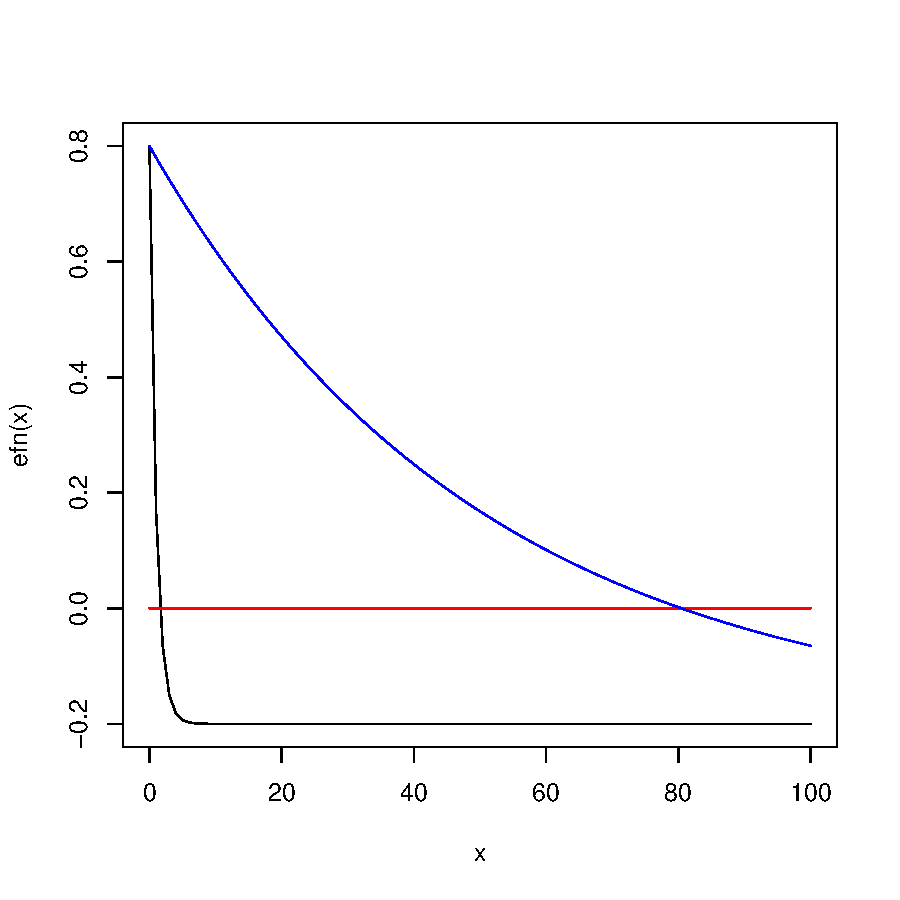
\includegraphics{roots-vig-chunk13}


\section{Approaches to solving 1D rootfinding problems}

From the above examples, it is clear that any rootfinder needs to tell the users what it
is intended to do. Unfortunately, few do make clear their understandings of a problem. And
users often do not read such information anyway! Let us consider the main ways in which
rootfinders could be called.

\begin{itemize}
\item{We could require the user to supply an interval -- a lower and upper bound
for a prospective root, and further insist that the function values at the ends of
the interval have opposite sign. This is the situation for 
\R's \texttt{uniroot} (\cite{brent73} and \texttt{root1d} (\cite{jncnm79}) 
from the package \texttt{rootoned}
at \url{https://r-forge.r-project.org/R/?group_id=395}.}
\item{An alternative approach is to consider that we will search for a root from
a single value of the argument $x$ of our function $f(x)$. This is the setup for 
a one-dimensional Newton's method, which iterates using the formula

$  x_{new} = x - f(x) / f'(x) $

}
\item{We may wish to specify the funtion with no starting value of the argument $x$. An
example is the \texttt{polyroot} function we have already used. As far as the author is
aware, there are no general rootfinders of this type in \R, or elsewhere to his 
knowledge.}
\end{itemize}

With \R, a possible package could be developed using an \textbf{expression} for the 
function. This would allow the symbolic differentiation operator \texttt{D()} to be 
applied to get the derivative, though there are some limitations to this tool. For
example, it does not comprehend \texttt{sum()} and other fairly common functions. I
have not bothered to pursue this possibility yet.

It is also possible to consider a secant-rule version of Newton's method. That is, we
use two points as in \texttt{zeroin}, \texttt{root1d} or \texttt{uniroot}, but do not
require that they have function values of opposite sign. An alternative setup would use
an initial guess to the root and a stepsize.

\section{What can go wrong?}

Rootfinding may seem like a fairly straightforward activity, but there are many 
situations that cause trouble.

\textbf{Multiple roots} are common for polynomial rootfinding problems. We already have
seen cases where the polynomial is a power of a monomial $(x-root)$. Computationally,
such problems are ``easy'' if we have an odd power and are using a rootfinder for
which we supply an interval that brackets the root. We will not, however, learn the
multiplicity of the root without further work. 

More troublesome are such problems when the function just touches zero, as when the
power of the monomial is even. In such case Newton's method can sometimes succeed,
but there is a danger of numerical issues if $f'(x)$ becomes very small, so that the
iteration formula blows up. In fact, Newton's methods generally need to be safeguarded
against such computational issues. Most of the code for a successful Newton-like 
method will be in the safeguards; the basic method is trivial but prone to numerical
failure.

Problems with no root at all, as in the example ``Not there'' above, require some
careful examination. Let us consider some example output, which has been edited to
avoid excessive space.

\begin{verbatim}
> tint<-c(80,100)
> ru<-uniroot(mytan, tint)
> ru: root= 90.00008, f.root=-750991.8, iter=19, estim.prec=7.63e-5

> rz<-zeroin(mytan, tint)
> rz: root=90, froot= -6152091027, rtol= 9.313226e-09, maxit= 30

> rr<-root1d(mytan, tint)
> rr: root= 100, froot=-5.671282, rtol= 0, count= 4

> rn<-newt1d(mytan, gmytan, aa, trace=TRUE)
1 :xold= 80  f= 5.671282  g= 0.5788112  xnew= 80 
1 :xold= 80  f= 5.671282  g= 0.5788112  xnew= 70.20184 
2 :xold= 70.20184  f= 2.777887  g= 0.1521344  xnew= 70.20184 
2 :xold= 70.20184  f= 2.777887  g= 0.1521344  xnew= 51.94241 
3 :xold= 51.94241  f= 1.277293  g= 0.04592796  xnew= 51.94241 
3 :xold= 51.94241  f= 1.277293  g= 0.04592796  xnew= 24.13161 
4 :xold= 24.13161  f= 0.4479839  g= 0.02095599  xnew= 24.13161 
4 :xold= 24.13161  f= 0.4479839  g= 0.02095599  xnew= 2.754241 
5 :xold= 2.754241  f= 0.04810763  g= 0.01749369  xnew= 2.754241 
5 :xold= 2.754241  f= 0.04810763  g= 0.01749369  xnew= 0.004241002 
6 :xold= 0.004241002  f= 7.401946e-05  g= 0.01745329  xnew= 0.004241002 
6 :xold= 0.004241002  f= 7.401946e-05  g= 0.01745329  xnew= 1.549063e-11 
7 :xold= 1.549063e-11  f= 2.703625e-13  g= 0.01745329  xnew= 1.549063e-11 
7 :xold= 1.549063e-11  f= 2.703625e-13  g= 0.01745329  xnew= -3.231174e-27 
8 :xold= -3.231174e-27  f= -5.639463e-29  g= 0.01745329  xnew= -3.231174e-27 
8 :xold= -3.231174e-27  f= -5.639463e-29  g= 0.01745329  xnew= 0 
> rn: root=0, froot=-5.639463e-29, itn= 8 
\end{verbatim}

Notes: 
\begin{itemize}
\item \texttt{root1d}, \texttt{zeroin}, \texttt{uniroot} don't give sufficient 
indication of trouble
\item \texttt{newt1d} goes to 0 degrees (another "root")
\end{itemize}

\section{Being a smart user of rootfinding programs}

Mostly -- and I am cowardly enough not to define ``mostly'' -- users of 
rootfinders like \texttt{uniroot} get satisfactory results without trouble. On the
other hand, it really is worthwhile checking these results from time to time. This
is easily done with the \texttt{curve} function that lets one draw the function of
interest. Examples above show how to add a horizontal line at 0 to provide a reference
and make checking the position of the root easy. Even within codes, it is useful to
generate a warning if the function value at the proposed root is ``large'', for
example, of the same order of magnitude as the function values at the ends of the
initial interval for the search. Indeed, I am surprised \texttt{uniroot} does not
have such a warning, and have put such a check into one of my own routines.

\section{Conclusions and extensions}

From the discussion above

\begin{itemize}
\item{Methods for univariate rootfinding work efficiently and well but still need
``watching''. This applies to almost any iterative computation.}
\item{There is a need for more ``thoughtful'' methods that give a user much more 
information about his or her function and suggest potential issues to be investigated. 
Such tools would be intended for use when the regular tools appear to be giving 
inappropriate answers.}
\item{As always, more good test cases and examples are useful to improve our methods.}
\end{itemize}


\bibliography{roots}


\end{document}
